\documentclass[a5paper, 10pt]{article}

% Текст
\usepackage[utf8]{inputenc} % UTF-8 кодировка
\usepackage[russian]{babel} % Русский язык
\usepackage{indentfirst} % красная строка в первом параграфе в главе
% Отображение страниц
\usepackage{geometry} % размеры листа и отступов
\usepackage{listings}
\usepackage{color}

\geometry{
	left=12mm,
	top=25mm,
	right=15mm,
	bottom=17mm,
	marginparsep=0mm,
	marginparwidth=0mm,
	headheight=10mm,
	headsep=7mm,
	nofoot}
\usepackage{afterpage,fancyhdr} % настройка колонтитулов
\pagestyle{fancy}
\fancypagestyle{style}{ % создание нового стиля style
	\fancyhf{} % очистка колонтитулов
	\fancyhead[LO, RE]{Лабораторная работа № 6 } % название документа наверху
	\fancyhead[RO, LE]{Задачи 1160, 1162, 1650} % название section наверху
	\fancyfoot[RO, LE]{\thepage} % номер страницы справа внизу на нечетных и слева внизу на четных
	\renewcommand{\headrulewidth}{0.25pt} % толщина линии сверху
	\renewcommand{\footrulewidth}{0pt} % толцина линии снизу
}
\fancypagestyle{plain}{ % создание нового стиля plain -- полностью пустого
	\fancyhf{}
	\renewcommand{\headrulewidth}{0pt}
}
\fancypagestyle{title}{ % создание нового стиля title -- для титульной страницы
	\fancyhf{}
	\fancyhead[C]{{\footnotesize
			Министерство образования и науки Российской Федерации\\
			Федеральное государственное автономное образовательное учреждение высшего образования
	}}
	\fancyfoot[C]{{\large 
			Санкт-Петербург, 2024
	}}
	\renewcommand{\headrulewidth}{0pt}
}

% Математика
\usepackage{amsmath, amsfonts, amssymb, amsthm} % Набор пакетов для математических текстов
%\usepackage{dmvnbase} % мехматовский пакет latex-сокращений
\usepackage{cancel} % зачеркивание для сокращений
% Рисунки и фигуры
\usepackage[pdftex]{graphicx} % вставка рисунков
\usepackage{wrapfig, subcaption} % вставка фигур, обтекая текст
\usepackage{caption} % для настройки подписей
\captionsetup{figurewithin=none,labelsep=period, font={small,it}} % настройка подписей к рисункам
% Рисование
\usepackage{tikz} % рисование
\usepackage{circuitikz}
\usepackage{pgfplots} % графики
% Таблицы
\usepackage{multirow} % объединение строк
\usepackage{multicol} % объединение столбцов
% Остальное
\usepackage[unicode, pdftex]{hyperref} % гиперссылки
\usepackage{enumitem} % нормальное оформление списков
\setlist{itemsep=0.15cm,topsep=0.15cm,parsep=1pt} % настройки списков
% Теоремы, леммы, определения...
\theoremstyle{definition}
\newtheorem{Def}{Определение}
\newtheorem*{Axiom}{Аксиома}
\theoremstyle{plain}
\newtheorem{Th}{Теорема}
\newtheorem{Lem}{Лемма}
\newtheorem{Cor}{Следствие}
\newtheorem{Ex}{Пример}
\theoremstyle{remark}
\newtheorem*{Note}{Замечание}
\newtheorem*{Solution}{Решение}
\newtheorem*{Proof}{Доказательство}
% Свои команды
\newcommand{\comb}[1]{\left[\hspace{-4pt}\begin{array}{l}#1\end{array}\right.\hspace{-5pt} } % совокупность уравнений
% Титульный лист
\usepackage{csvsimple-l3}
\newcommand*{\titlePage}{
	\thispagestyle{title}
	\begingroup
	\begin{center}
		%		{\footnotesize
			%			Министерство образования и науки Российской Федерации\\
			%			Федеральное государственное автономное образовательное учреждение высшего образования
			%		}
		%		
		\vspace*{6ex}
		
		{\small
			САНКТ-ПЕТЕРБУРГСКИЙ НАЦИОНАЛЬНЫЙ ИССЛЕДОВАТЕЛЬСКИЙ УНИВЕРСИТЕТ ИТМО	
		}
		
		\vspace*{2ex}
		
		{\normalsize
			Факультет систем управления и робототехники
		}
		
		\vspace*{15ex}
		
		{\Large \bfseries 
			Лабораторная работа № 6
		}
\vspace*{2ex}
	{\Large \bfseries 
			
"Задачи 1160, 1162, 1650"
		}
\vspace*{2ex}
		
		{\normalsize
			по дисциплине Алгоритмы и структуры данных
		}

	\end{center}
	\vspace*{20ex}
	\begin{flushright}
		{\large 
			\underline{Выполнила}: студентка гр. \textbf{R3238}\\
                             поток \textbf{2.1}\\
			\begin{flushright}
				\textbf{Нечаева А. А.}\\
			\end{flushright}
		}
		
		\vspace*{5ex}
		
		{\large 
			\underline{Преподаватель}: \textit{Тропченко Андрей Александрович}
		}
	\end{flushright}	
	\newpage
	\setcounter{page}{1}
	\endgroup}

\begin{document}
	\titlePage
	\pagestyle{style}

\lstset{ %
language=C,                 % выбор языка для подсветки (здесь это С)
basicstyle=\small\sffamily, % размер и начертание шрифта для подсветки кода
numbers=left,               % где поставить нумерацию строк (слева\справа)
numberstyle=\tiny,           % размер шрифта для номеров строк
stepnumber=1,                   % размер шага между двумя номерами строк
numbersep=5pt,                % как далеко отстоят номера строк от подсвечиваемого кода
backgroundcolor=\color{white}, % цвет фона подсветки - используем \usepackage{color}
showspaces=false,            % показывать или нет пробелы специальными отступами
showstringspaces=false,      % показывать или нет пробелы в строках
showtabs=false,             % показывать или нет табуляцию в строках
frame=single,              % рисовать рамку вокруг кода
tabsize=2,                 % размер табуляции по умолчанию равен 2 пробелам
captionpos=t,              % позиция заголовка вверху [t] или внизу [b] 
breaklines=true,           % автоматически переносить строки (да\нет)
breakatwhitespace=false, % переносить строки только если есть пробел
escapeinside={\%*}{*)}   % если нужно добавить комментарии в коде
}



\newpage
\section{Цель}
Разработать и реализовать алгоритмы для решения задач 1160, 1162 и 1650.


\section{Задача 1160}

\begin{figure}[h]
\center{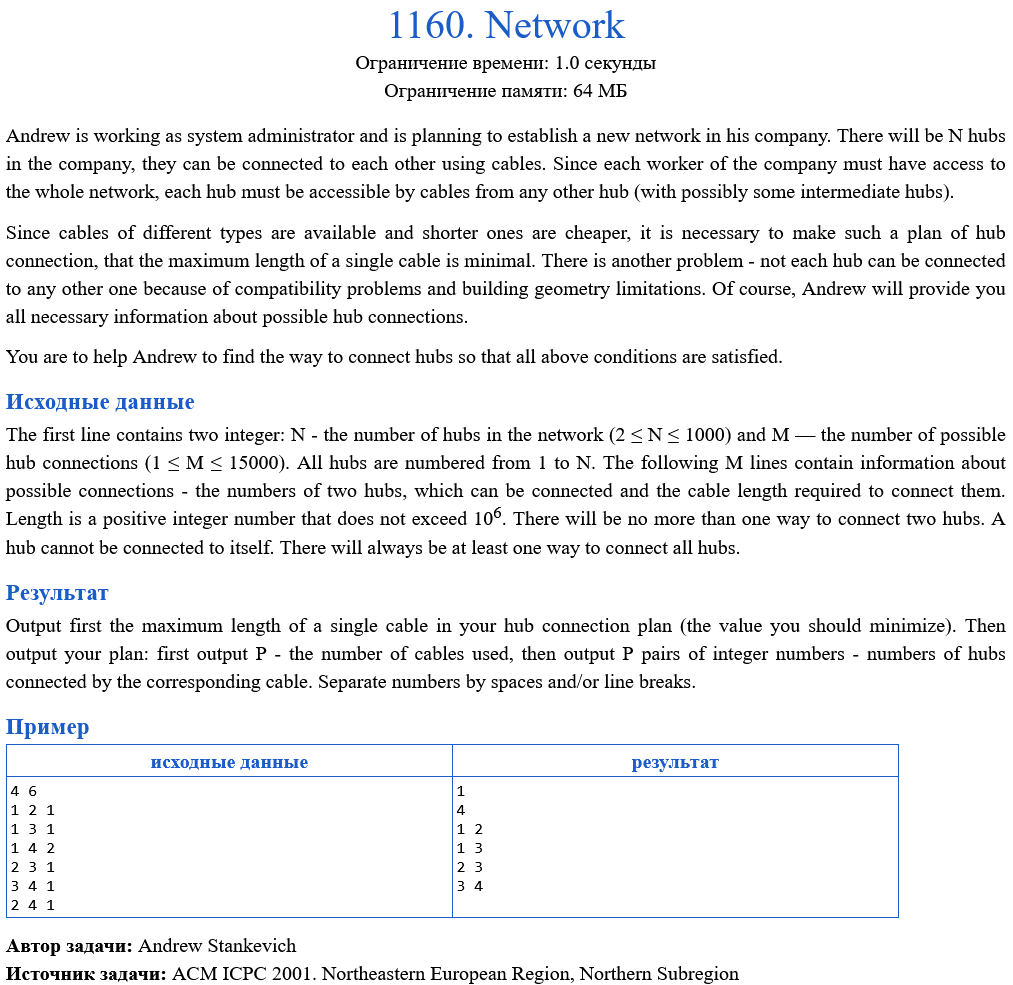
\includegraphics[width=0.9\linewidth]{pic/task_1160.png}}
\caption{Условие задачи 1160.}
\end{figure}

\subsection{Краткое описание алгоритма}
В основе реализации лежит алгоритм \textbf{Краскала} -- алгоритм поиска минимального остовного дерева (англ. \textit{minimum spanning tree, MST}) во взвешенном неориентированном связном графе.\\

Идея алгоритма Краскала: последовательное построение подграфа $F$ графа $G$, стремясь на каждой итерации достроить $F$ до $MST$. Включим в $F$ все вершины $G$. Перейдем к обходу множества ребер графа $G$ в порядке неубывания весов ребер. Если какое-то ребро соединяет вершины одной компоненты связности $F$, то оно не может быть включено в $F$, так как при его добавлении возникнет цикл. Иначе добавляем это ребро в $F$. На последней итерации ребро объединит две компоненты связности, полученный подграф будет минимальным остовным деревом графа $G$.\\


\textbf{1. Входные данные:} в первой строке содержится два целых числа: $N$ $-$ число хабов в сети $(2 \leq N \leq 1000)$ и $M$ $-$ число возможных соединений хабов $(1 \leq M \leq 15000)$. Все хабы имеют номера от 1 до $N$. Следующие $M$ строк содержат информацию о возможных соединениях $-$ номера двух хабов, которые могут быть соединены кабелем, и длину соответствующего кабеля.\\
\textbf{2.}  Зададим структуру для соединения (начальный хаб, конечный и длина кабеля). При считывании данных будем записывать все соединения в структуру данных \textit{std::vector}. Отсортиуем полученный вектор по неубыванию.\\
\textbf{3.}  Теперь добавляем соединения (ребра в граф), вершины обозначаем такими номерами, которые соответствуют номерам подграфов, не соединенных с другими подграфами.\\
\textbf{4.}  Если мы объединяем два подграфа, то присваиваем объединению наименьший из исходных номеров компонент. В конце все вершины должны оказаться соединенными.\\
\textbf{5. Выходные данные:} вывести максимальное значение длины кабеля в полученном плане соединений (значение, которое нужно минимизировать). Далее вывести количество использованных кабелей и вывести пары, соединенных хабов.

\newpage
\subsection{Листинг}

\begin{center}
\begin{lstlisting}[label=some-code,caption={Исходный код для 1160}]
#include <iostream>
#include <algorithm>
#include <vector>


// special structure to store information about connections
struct _connection {
    int v_1;
    int v_2;
    int l;
};

// special comparator to sort possible connections
bool _compare(_connection c_1, _connection c_2) {
    return c_1.l < c_2.l;
}



int main(){

    int N, M, v_1, v_2, l;
    std::cin >> N >> M;
    // vector of possible connections
    std::vector<_connection> _pos_con;

    for (int i = 0; i < M; ++i) {

        std::cin >> v_1 >> v_2 >> l;
        _pos_con.push_back((_connection){v_1 - 1, v_2 - 1, l});
    }
    // here starts the Kruskal's algorithm
    std::sort(_pos_con.begin(), _pos_con.end(), _compare);

    int _visited_v[N];
    int _visited_e[M];

    for (int i = 0; i < N; ++i) {
        _visited_v[i] = -1;
    }

    for (int i = 0; i < M; ++i) {
        _visited_e[i] = 0;
    }

    int _subgraph_number = 0;
    int _max = 0;
    int _counter = 0;

    for (int i = 0; i < M; ++i) {
        if (_visited_v[_pos_con[i].v_1] != -1 && _visited_v[_pos_con[i].v_1] == _visited_v[_pos_con[i].v_2]) continue;

        else if (_visited_v[_pos_con[i].v_1] == -1 && _visited_v[_pos_con[i].v_2] == -1) {
            _visited_v[_pos_con[i].v_1] = ++_subgraph_number;
            _visited_v[_pos_con[i].v_2] = _subgraph_number;

        } else if ((_visited_v[_pos_con[i].v_1] != -1 && _visited_v[_pos_con[i].v_2] == -1) ||
                   (_visited_v[_pos_con[i].v_1] == -1 && _visited_v[_pos_con[i].v_2] != -1)) {

            int _loc_subgraph = _visited_v[_pos_con[i].v_1] + _visited_v[_pos_con[i].v_2] + 1;
            _visited_v[_pos_con[i].v_1] = _loc_subgraph;
            _visited_v[_pos_con[i].v_2] = _loc_subgraph;
        } else {

            int min_subgraph;
            int max_subgraph;

            if (_visited_v[_pos_con[i].v_1] < _visited_v[_pos_con[i].v_2]) {
                min_subgraph = _visited_v[_pos_con[i].v_1];
                max_subgraph = _visited_v[_pos_con[i].v_2];
            } else {
                max_subgraph = _visited_v[_pos_con[i].v_1];
                min_subgraph = _visited_v[_pos_con[i].v_2];
            }

            for (int j = 0; j < N; ++j) {
                if (_visited_v[j] == max_subgraph) {
                    _visited_v[j] = min_subgraph;
                }
            }
        }
        _visited_e[i] = 1;
        _max = _pos_con[i].l;
        ++_counter;

    }
    std::cout << _max << std::endl << _counter << std::endl;

    for (int j = 0; j < M; ++j) {
        if (_visited_e[j]) {
            std::cout << _pos_con[j].v_1 + 1 << " " << _pos_con[j].v_2 + 1 << std::endl;
        }
    }

    return 0;

}


\end{lstlisting}
\end{center}

\subsection{Результат}
\begin{figure}[h]
\center{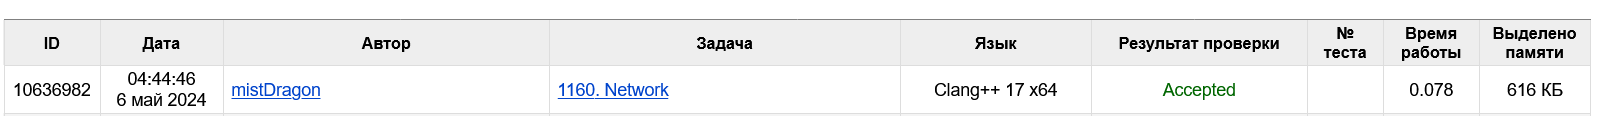
\includegraphics[width=0.9\linewidth]{pic/screen_1160.png}}
\caption{Результат отправки задачи 1160.}
\end{figure}



\newpage
\section{Вывод по работе}
В ходе выполнения данной лабораторной работы были реализованы алгоритмы для решения задач $1160$, $1162$ и $1650$. \\

Решение задачи 1160 основывается на применении алгоритма Краскала.
\end{document}













